\chapter{Architecture and Design of DRS}
\label{chap:design}

\section{Functions of DRS}
Distributed resource scheduler is responsible for handling the dynamic resource allocation requirements of VMs on the cloud. The job of a DRS can be divided into three categories:

\begin{enumerate}
\item \textbf{Monitoring.} Monitoring is essential for detecting the resource requirements of individual guest machines running on the cloud and detecting hotspots on physical hosts which make up the cluster. It has to be fine-grained enough to detect changes in the load profile of the hosts and guests. It has to be coarse enough to filter short-terms changes in the resource requirements of the guests. It will also regularly update the load statistics of the host in a shared data store which can be used to get a global account of the cluster state at any point of time which will be useful in making decisions about live-migration.
\item \textbf{Memory Management.} For all the guests running on the same host, DRS will manage their ever changing memory demands. Autoballooning is an essential technique for the DRS to perform this aspect of its functionality. This part of DRS will look at the memory usage statistics of all the guests, figure out which VMs need more memory and which VMs have idle memory, and try to meet the demands of each VM by inflating/deflating its balloon.
\item \textbf{Hotspot Mitigation.} In the case of a hotspot, this part of DRS is responsible for selecting an appropriate guest to migrate and the best destination for it based on the resource usage data of all the machines present in the cluster.
\end{enumerate}

\section{Goals and Non-Goals}
\textit{Goal:} Develop a DRS for private clouds which makes the best use of the resources available i.e. provides the resources to the machines on a best effort basis according to the priority/importance of each VM. If the cluster is not fully loaded, the demands of all the VMs can be satisfied but if the load is more than the capacity, the VMs will have to do with less resources than promised. In case of an overload, all the VMs with the same priority across the cluster should be treated equally in resource allocation. 

\textit{Goal:} The DRS design should be decentralized so that it is easily able to scale up to a cluster having thousands of physical hosts and there is no single point of failure in the system.

\textit{Non-goal:} Minimizing the number of machines used. Though using less machines will save power because the unused machines can be turned off, the goals of power management are orthogonal to the goals of our DRS and can be treated separately.

\textit{Non-goal:} For the purpose of this thesis, we have considered balancing only memory and CPU resources. Other resources like disk I/O, and network bandwidth have not been taken into account.

\section{Architecture Overview}
%TODO: insert a figure here.
The DRS architecture described below is fully decentralized, which is a key requirement for scaling it up to thousands of hosts. Decentralization also prevents any single point of failures. Each host in the cluster makes its own decision about the guest machines on that host and the other hosts co-operate with it to make that decision successful.
The DRS is divided into three components based on the three types of job mentioned earlier that it has to perform. 

\begin{figure}[!ht]
  \centering
  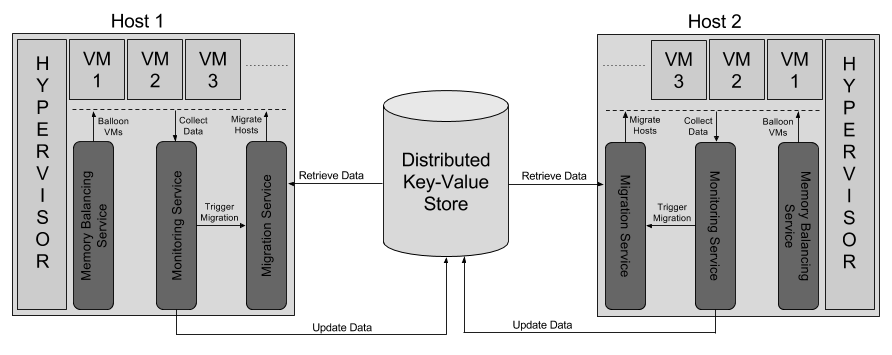
\includegraphics[width=\textwidth]{arch.png}
  \caption{Architecture of the DRS}\label{fig:mem}
\end{figure}

\subsection{The Monitoring Service}
A \textit{monitoring service} runs on all the hosts of the cluster. On each host, it collects the resource usage statistics of all the VMs on the host and the total resource usage of the host. It also filters out the short-term changes in the resource usage and figures out the changes in the load profile. It also detects any hotspot and triggers the migration service to perform its task of migrating a guest away from the host. The service also accommodates (start monitoring) any new guest that is migrated to a host. 

The service talks to a distributed key-value store to regularly update the resource usage statistics of the host it is running on. The key-value store should be updated only when there is a significant change in the resource usage profiles of the host, which could affect the decision making of live migration. Small changes in the resource usage are unnecessary to track as they will not affect the decision making. Short-term spikes in the resource usage can adversely affect the live-migration decisions by misrepresenting the resource usage.

\subsection{The Memory Balancing Service}
A \textit{memory balancing Service} runs on all the hosts. On each host, the service looks at the memory usage statistics of all the VMs running on the host provided by the monitoring service. It figures out which hosts require more memory and which hosts have some idle memory. It then balances the memory by inflating/deflating the balloons of the VMs.

If the demands of all the VMs can be satisfied, balancing takes idle memory and gives it to the needy. If the demands of all the VMs cannot be satisfied i.e. there is a hotspot on the host, the service calculates the entitled memory based on the priority of each VM running on the host for each guest. Entitled memory may be less than the memory needs of a guest. Then the service distributes memory according to the entitlement. 

The service also tries to make space by freeing memory for any new guest that is to be migrated to the host. Notably, this service does not do anything to resolve hotspots. It just tries to balance memory amongst the guests present on the host. Hotspot mitigation is left to the migration service. If there is a hotspot, some guest(s) may get migrated out of the host, leaving free memory for other VMs.

The memory management requires a separate service while CPU management does not. There are two reasons for this.
\begin{enumerate}
\item vCPU of each VM is handled as a thread by the hypervisor and hence scheduled according to its process scheduling policy, while there is no such system for memory.
\item Memory, once consumed by a VM, is not reclaimed automatically by the hypervisor, while this is not the case with the CPU resources. Each vCPU thread gets a time slice to run which is decided by the hypervisor and the CPU is taken away from the thread after the time slice ends.

\end{enumerate}

\subsection{The Migration Service}
This service runs on all the hosts and is triggered by the \textit{monitoring service} when there is a hotspot on the host. It collects the resource usage statistics of all the other hosts in the cluster from the data-store to which the monitoring services of all the hosts write. This data would be just a few key-value pairs per host and hence, very small. Using this data (and some other), it tries to find out the best migration (guest VM-destination host pair) performing which will improve some metric representing the resource requirement satisfaction or the overall performance of the VMs on the cluster. The service talks to the memory balancing service on the destination host to free required memory for the incoming guest, and then it migrates the guest to the destination. The migration service requires resource usage details of the entire cluster to make an informed decision on migration.

\subsection*{Summary}
In this chapter, we have discussed the functions and goals of a DRS. We have also proposed a decentralized architecture for DRS which can scale well and is free of single point failures.